\documentclass{standalone} 
\usepackage{tikz}
\usetikzlibrary{positioning, shapes, automata, arrows}
\usetikzlibrary{shapes.geometric}
\usepackage{pgfplots}
\usepackage{latexsym}
\usepackage{algorithm}
\usepackage{algorithmic}
% \pgfplotsset{compat=latest}
\usepackage{amsmath}
\usepackage[varg]{txfonts}
\usepackage{pgfplotstable}
\usetikzlibrary{patterns}
\def\minYear{1987}
\def\maxYear{2014}
\def\xmin{\minYear-1900-0.5}
\def\xmax{\maxYear-1900+0.5}
\pgfplotsset{compat=1.13}  % PGFPlots 1.13の機能セットを使用することを宣言
% used PGFPlots v1.14
% \documentclass[border=5pt]{standalone}
% \usepackage{pgfplots}
\newcommand{\A}{DV} 
\newcommand{\B}{Unknown} 
\usetikzlibrary{
       patterns,
}
       \pgfplotsset{
           compat=1.7,
           % define your own legend style here
           my ybar legend/.style={ 
             legend image code/.code={
               \draw [##1] (0cm,-0.6ex) rectangle +(2em,1.5ex);
               },
           },
       }
\begin{document}
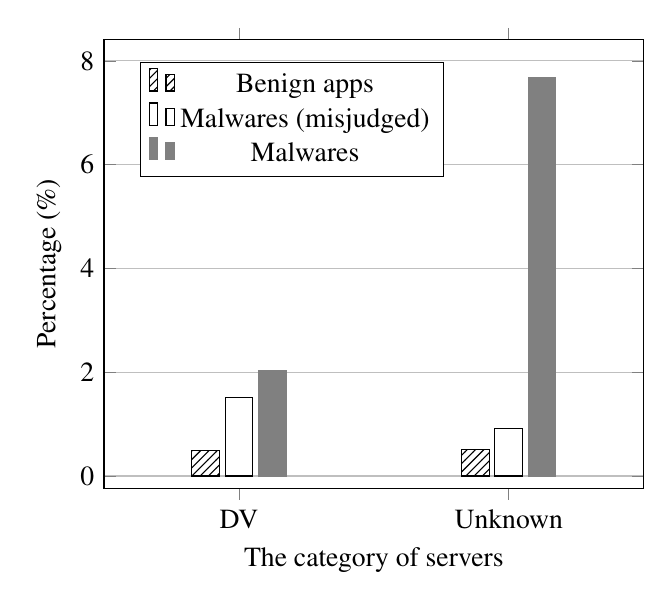
\begin{tikzpicture}
  \begin{axis}[
    ylabel=Percentage (\%),
    xlabel=The category of servers,
    % enlarge x limits=0.2,
    % area legend, % 長方形の凡例
    legend style={ % 凡例の位置
      at={(0.63,0.95)},
      % anchor=north,legend columns=-1
    },
    % ymin=0,
    ybar,
    xtick=data,
    % bar width=0.3, % 棒グラフの幅
    symbolic x coords={0, 0.1, \A,0.4, 0.5, 0.6, \B, 0.9, 1},
    ymajorgrids = true,
    xmin=0, xmax=1, % x軸方向の範囲
    % xmajorgrids=false
    ]

    \addplot [pattern=north east lines] coordinates {(\A, 0.487) (\B, 0.518) };
    % \addplot [] coordinates {(\A, 1.202) (\B, 2.072)};
    \addplot [] coordinates {(\A, 1.516) (\B, 0.916)};
    \addplot [gray, fill] coordinates {(\A, 2.039) (\B, 7.688)};
    \legend{Benign apps, Malwares (misjudged), Malwares}
  \end{axis}
\end{tikzpicture}
\end{document}

% \begin{document}
% \begin{tikzpicture}
% \scriptsize
% \begin{axis}[
% width=1.9in,
% height=1.5in,
% scale only axis,
% ymin=0,
% enlarge x limits={abs=0.5},
% bar shift auto,
% legend pos=north west,
% table/row sep=crcr,
% ybar,
% bar width=0.3,
% symbolic x coords={Benign, Malwares},
    % % apply your own legend style here (or at each '\addplot command)
    % my ybar legend,
    % ]

    % \addplot [pattern=north east lines] table {
        % Benign   0.489\\
        % % 2   3\\
        % Malwares   0.510\\
      % };
    % % \addplot [pattern=dots] table {
    % % 1   2\\
    % % 2   3\\
    % % 3   4\\
    % % };
    % \addplot [] table {
        % Benign   1.630\\
        % % 2   3\\
        % Malwares   12.994\\
      % };
    % \legend{
      % DV,
      % % Second,
      % Unknown,
    % };
% \end{axis}
% \end{tikzpicture}
% \end{document}
